\documentclass[sigconf]{acmart}



%% Packages
\usepackage[acronym,toc,nonumberlist]{glossaries}
\usepackage[inline]{enumitem}
\usepackage[anythingbreaks]{breakurl}

%%
%% Hyphenation rules adding a bit more human intel to stupid latex
\hyphenation{data-bases}

%%
%% Commands for first letter bold
\newcommand{\fb}[1]{\dofb#1}
\newcommand{\dofb}[1]{\textbf{#1}\nobreak\hspace{0pt}}

%%
%% The majority of ACM publications use numbered citations and
%% references.  The command \citestyle{authoryear} switches to the
%% "author year" style.
%%
%% If you are preparing content for an event
%% sponsored by ACM SIGGRAPH, you must use the "author year" style of
%% citations and references.
%% Uncommenting
%% the next command will enable that style.
%% \citestyle{acmauthoryear}

%%
%% Glossaries
\makeglossaries
%% Use TOC dots. Not used anymore, as page numbers were killed
%% \renewcommand*\glspostdescription{\cftdotfill{\cftdotsep}}
%% Add support for tree glossaries
%% \renewcommand{\glossarypreamble}{\glsfindwidesttoplevelname[\currentglossary]}
%% Number of columns for mcols
%% \renewcommand{\glsmcols}{2}
\newacronym{dbms}{DBMS}{database management system}
\newacronym[shortplural={DDBS}]{ddbs}{DDBS}{distributed database system}


%%
%% Commalist
\newlist{commalist}{enumerate*}{1}
\setlist[commalist]{
    label=(\arabic*),
    itemjoin={{, }},
    itemjoin*={{, and }},
    afterlabel=\unskip{{~}}
}

\newlist{commalistor}{enumerate*}{1}
\setlist[commalistor]{
    label=(\arabic*),
    itemjoin={{; }},
    itemjoin*={{; or }},
    afterlabel=\unskip{{~}}
}

%%
%% Break URLs on dashes
\def\UrlBreaks{\do\/\do-}



\begin{document}

\title{Praktikum: Cloud Data Bases\\Final Report}


\author{Aly Kamel}
\authornote{Authors contributed equally to this work.}
\email{aly.kamel@tum.de}
\affiliation{%
\institution{Technical University of Munich}
}
\author{Iremnur Kidil}
\authornotemark[1]
\email{ge34hoz@tum.de}
\affiliation{%
\institution{Technical University of Munich}
}
\author{Ricardo Kraft}
\authornotemark[1]
\email{...}
\affiliation{%
\institution{Technical University of Munich}
}



\renewcommand{\shortauthors}{Kamel}
\renewcommand{\shortauthors}{Kidil}
\renewcommand{\shortauthors}{Kraft}

% !TeX root = ../main.tex

% TODO: outline

\begin{abstract}
    Today, almost
\end{abstract}


\begin{CCSXML}
	<ccs2012>
	<concept>
	<concept_id>10010520.10010553.10010562</concept_id>
	<concept_desc>Computer systems organization~Embedded systems</concept_desc>
	<concept_significance>500</concept_significance>
	</concept>
	<concept>
	<concept_id>10010520.10010575.10010755</concept_id>
	<concept_desc>Computer systems organization~Redundancy</concept_desc>
	<concept_significance>300</concept_significance>
	</concept>
	<concept>
	<concept_id>10010520.10010553.10010554</concept_id>
	<concept_desc>Computer systems organization~Robotics</concept_desc>
	<concept_significance>100</concept_significance>
	</concept>
	<concept>
	<concept_id>10003033.10003083.10003095</concept_id>
	<concept_desc>Networks~Network reliability</concept_desc>
	<concept_significance>100</concept_significance>
	</concept>
	</ccs2012>
\end{CCSXML}

\maketitle

\section{Introduction}
\label{sec:introduction}

One of the main criteria when developing a key-value database(DB), is being able to handle large amounts of data while making the system available for multiple clients. DB systems, such as AmazonWeb Services, Microsoft Azure SQL and Oracle Database offer the combination of scalability and cost effectiveness.

Another important feature is elasticity which measures the ability of a system to dynamically scaled up or down. The key-value DB BigTable and PNUTS are great examples\cite{agrawal2011database}.

Amazon DynamoDB is a non-relational database system which provides single-digit millisecond latency \cite{amazon}, considering the system is used worldwide. Data records are stored with a primary or composite key and several attributes depending on client's request \cite{kalid2017big}. 

Apache Cassandra is another key-value based high scaled \cite{abadi2012consistency} DB system, which is known for managing some of the world's largest datasets on clusters with the help of thousands of nodes distributed amongst multiple data centres \cite{chebotko2015big}. Cassandra offers more flexibility regarding fault handling and managing wide range data, unlike BigTable and Dynamo \cite{kalid2017big}. The system focuses on high level of availability by scaling millions of read and write requests per second\cite{chebotko2015big}.

Our inspiration mainly came from the DB Redis. It rose in popularity after its creation in 2009 and got deployed by many big companies such as Instagram \cite{krieger2011instagram} and Twitter \cite{yu2014twitter}, which require enormous DBs and fast responses to the millions of users they serve. One of its multiple features is the Pub/Sub system \cite{redis2020pubsub}, added in March 2010 \cite{sanfilippo2010pubsub}. With it, clients are able to subscribe to a set of keys, namely topics, and receive an update whenever their associated values get overwritten. In this model, clients keep waiting for the server to send them an update. During that period, subscribers are expected to use only subscription related operations.

In our system, we wanted for there to be no distinction between publishers and subscribers with everyone being able to both publish and receive updates. Apart from that, access to the DB should still be possible. 

Thus, the way we modelled our system in the end, was having a many-to-many relationship of all subscribed clients, effectively, implementing a group chat functionality.



\section{Background}
\label{sec:background}
In this section, we elaborate on some of the basic concepts that our key-value system depends on. First, we discuss the CAP theorem and analyse where our system lies on that spectrum. Then, we mention two design paradigms, namely BASE and ACID, and explain the differences between them.

\subsection{Key-value store}
Key-value stores are perhaps the simplest type of a NoSQL DB. Every information is saved in the form of key value pairs. Typically the key’s memory space is very small compared to the one of the values. The key is used as an identifier to the actual data saved in the value. The client will always need to have a key in order to work with the DB. 

In our case values are limited to strings and can be easily stored and retrieved just by providing the corresponding key, which is also limited to a string.


\subsection{Persistence}
%TODO add how data gets stored on disk

\subsection{Caching}
write through policy

\subsection{CAP Theorem}
\label{sec:background_cap} 
According to the CAP Theorem, distributed databases have three substantial properties to consider: consistency, availability and partition tolerance\cite{brewer2012cap}. Eric Brewer, the man behind the CAP theorem, stated that a distributed database can fulfil at most two of three properties\cite{brewer2000cap}:

\begin{itemize}
  \item Consistency: \\
  Clients are provided with fresh data, meaning the most up-to-date version of the data that got stored after the last write operation.
  \item Availability: \\
  Servers respond to the request of clients at all cases. Every non-failing node in the system must be able to serve the client in a reasonable amount of time\cite{gilbert2002brewer}.
  \item Partition tolerance: \\
  Whenever a server crashes, the rest of the system will still stay functional after the crash, without any information being lost.
\end{itemize}

Twelve years after from proposing the CAP theorem, Brewer mentioned that software engineers do not have to strictly abide to the 2 of 3 principle, it is rather a spectrum than a binary choice \cite{brewer2012cap}. In other words, a distributed DBS can favour high level of consistency and partition tolerance by having low level of availability. Thus, the initial theorem is improved by not having to sacrifice availability completely in this case.

There are two design approaches for distributed database systems, namely ACID and BASE. According to Brewer, these two design approaches may be referred as opposites of each other\cite{brewer2012cap} because of their priorities and use cases. ACID approach is used most of the times for relational database systems (SQL) and focuses on consistency to maintain reliability. On the contrary BASE is more suitable for the non-relational database systems (NoSQL) concentrating on providing the client high level of availability\cite{brewer2000cap}.

\subsection{ACID}
\label{sec:background_acid}
ACID is a traditional design approach\cite{brewer2012cap} when it comes to large-scaled distributed systems. The main goal of ACID is that despite the system having partitions, the client should always be provided with consistent values. It is an acronym which stands for the four following properties:
\begin{itemize}
\item Atomicity:\\
A set of transactions succeed all at once or fail all together. In other words, it is an all or nothing strategy.
\item Consistency: \\
The system never contains any stale data. When a client wants to read from any server, the returned value must be the value from the last write commit by any client. All clients should always get the same result whenever they try to fetch the same information.
\item Isolation:\\
All transactions happen isolated from each other and do not affect each other. Thus, if one transaction fails, all others are undisturbed.
\item Durability:\\
Once a client is informed that a transaction has been successfully committed, even if a crash occurs, the transaction would still stay committed.
\end{itemize} 

\subsection{BASE}
\label{sec:background_base}
BASE, another design approach defined by Brewer, offers looser requirements than ACID\cite{brewer2012cap}. Non-relational database systems concentrating on high availability make use of the BASE approach, which sacrifices strong consistency in favour of being always accessible. Examples include huge storage services such as Amazon's Dynamo, Facebook's Cassandra or Google's BigTable, where millions of active users always expect the service to be available\cite{kalid2017big}. Nevertheless, there must be trade-offs. By not guaranteeing the consistency at all time, the system cost is reduced, and clients are happier, but a client might not get an immediate response to his request.

\begin{itemize}
  \item Basic Availability:\\
 Clients are guaranteed to get a quick response from the server without getting blocked, however the returned value may be stale, stated in other words, inconsistent with the latest version.
  \item Soft State:\\
Since stale data is permitted, servers never truly know whether they are currently up-to-date or if they still contain invalid data.
  \item Eventual Consistency:\\
If there are no updates in the system for a long time, then all servers will gradually become consistent. Since the time is not specified, servers are always in a soft state, as explained above.
\end{itemize}

    


\section{Key-value server}
 Before we get into the details of milestone 5, we would like to revisit the implementation of the distributed key-value storage system we were tasked to develop and briefly discuss some of its features. Figure \ref{fig:ms4_arch} displays how a client interacts with its Connection Handle Thread (CHT), the helper thread assigned to serve it. In the following sections, we take a deeper look at how the client side and storage system visible in \ref{fig:ms4_arch} are structured and how they function.

\begin{figure}[h]
	\centering
	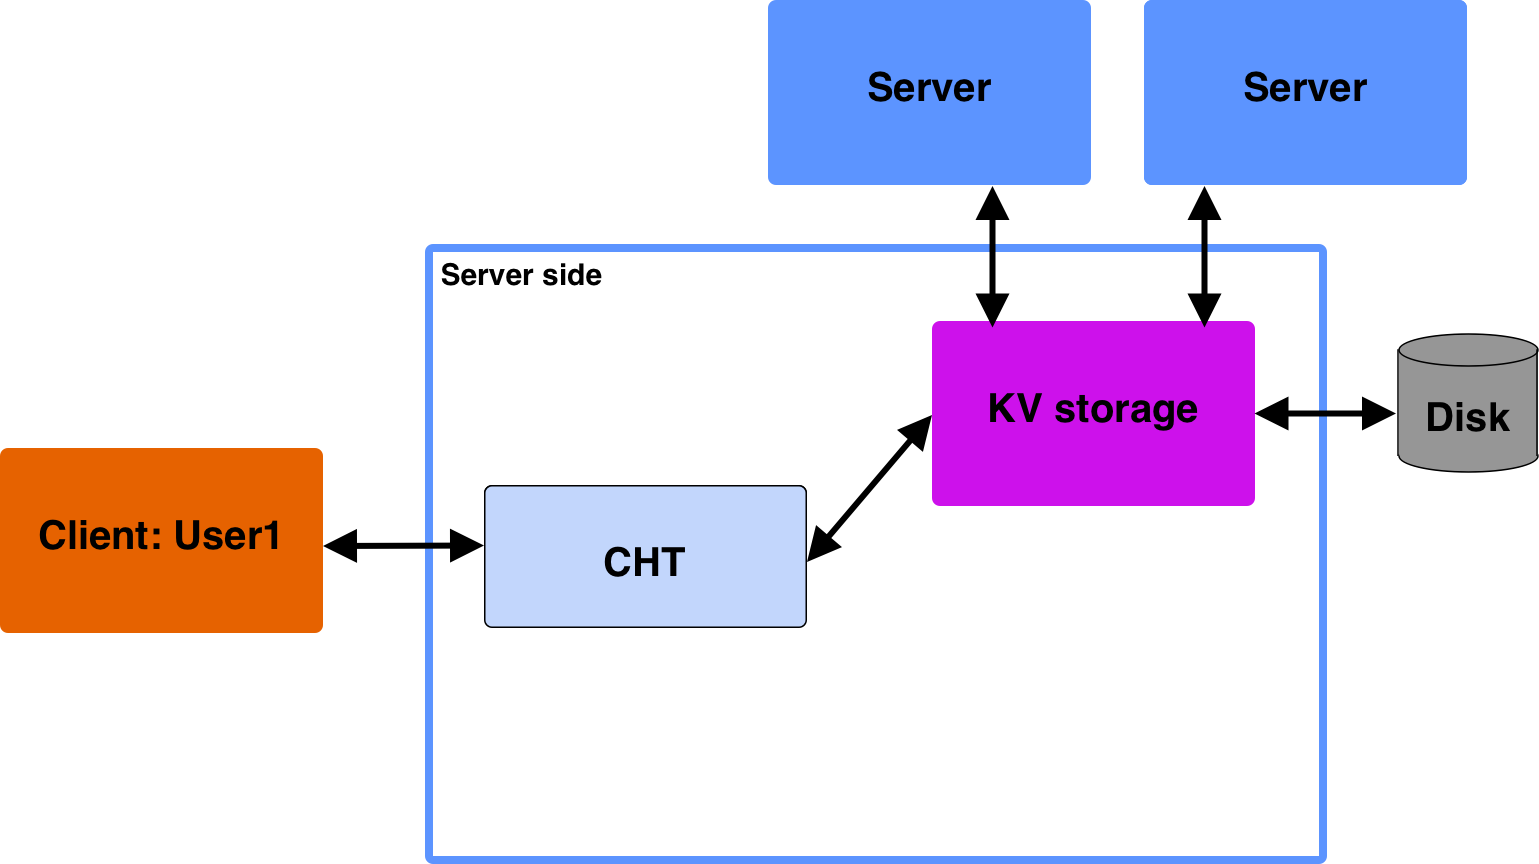
\includegraphics[width=\linewidth]{figures/kvserver/ms4_structure.png}
	\caption{Key-value server architecture}
	\label{fig:ms4_arch}
\end{figure}



%Client Side
\subsection{Client side}

\begin{figure}[h]
	\centering
	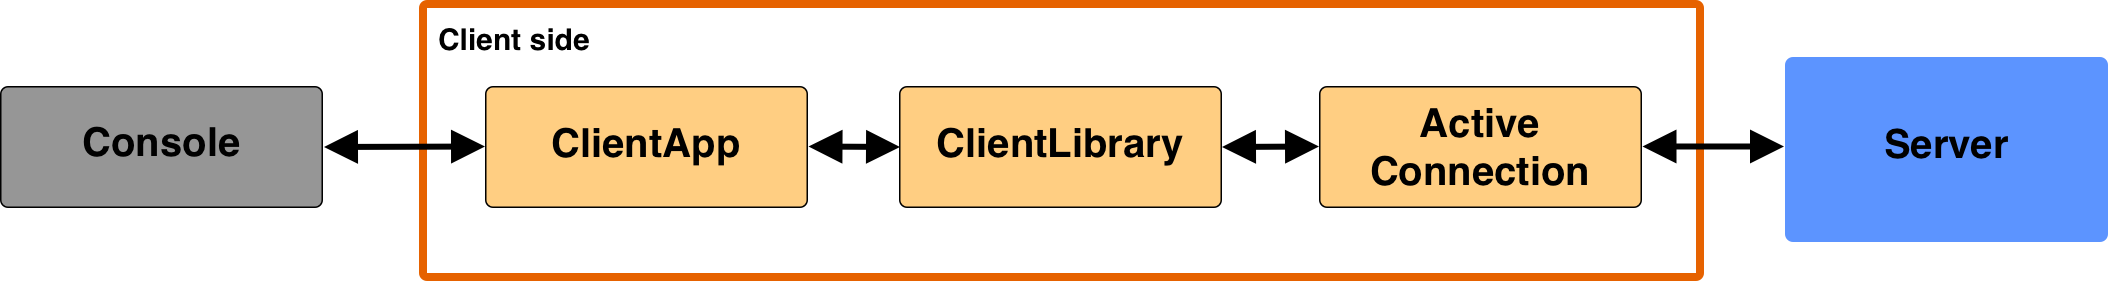
\includegraphics[width=\linewidth]{figures/kvserver/client_arch.png}
	\caption{Client side architecture}
	\label{fig:client_arch}
\end{figure}

The client side consists of the three following main components as seen in figure \ref{fig:client_arch}:

\begin{enumerate} 
  \item \textit{ClientApp}: represents the client interface which allows input through the console. From there the client is able to issue commands to connect to and disconnect from the system, interact with the key-value store and chat. The input is then checked and parsed before getting sent to the ClientLibrary. The result of the user's request gets displayed on the console through the ClientApp.
  \item \textit{ClientLibrary}: serves as a bridge between the client and the server. It contains an instance of the hash ring and is responsible to connect to the correct server.
  \item \textit{ActiveConnection}: abstracts the TCP socket connection to the server which allows the client to exchange data with the CHT without worrying about the underlying structure.
\end{enumerate}
 
 % Server side
\subsection{Server side}
\label{sec:server_side}

As previously mentioned, the CHT waits on the socket for the client to send a request. Afterwards, the request is forwarded to the key-value processor (KVP), which parses the client's string and translates it into direct DOPs. Then the ServerRing, which contains information about the hash ring, is called to check whether the current server is responsible for performing the requested operation on the provided key or not. In the former case, the request gets transferred to the KVStore. There, the read operations get passed on to the cache. In case of a cache miss, the requests gets redirected to the DiskStore. Write operations are instead always passed to the cache, the DiskStore and the Replication Manager (RPM). We use a write-through cache, which means write operations always get instantly sent to the cache, as mentioned in \ref{sec:caching}.

Upon starting the server, the DiskStore creates a directory containing three subdirectories. One for storing the keys it has write access to and one for each of the key sets it has only read access to. The second type of folders are called replica folders. A file in our system represents a key-value pair with the key being the file name and the value the file content.
The RPM is in charge of both sending updates to the server's replicas and receiving updates sent by the responsible servers.

As of milestone 4, replication is added to the system with the intention of increasing the availability by distributing the data records to the two replica servers and reducing therefore the latency of DOPs. Eventual consistency is achieved due to the fact that servers automatically forward all write operations to their replicas. Even if it takes a long time, all replicas will eventually contain the identical information as the original server. In order to maintain strong consistency as described in \ref{sec:background_acid}, a client performing a \texttt{PUT} operation would have to also wait until the value gets sent over to both of the servers replicas, which would result in slower \texttt{PUT}s. Since our system is not designed to handle important real-time transactions such as in a banking system, eventual consistency satisfies our database needs while allowing faster response times and higher availability. Persisting data permanantly on disk, however, means that we meet the durability goal of the ACID model.
Since the implementation of milestone 3, it is possible to monitor key-value stores continuously. The ECS pings each server every 700 milliseconds to be informed about the server's availability. If a server does not respond to the ping within a given time period, it is considered shutdown. However, due to the redundancy of replication,
up to two simultaneous failing server nodes can be tolerated, thus partition tolerance is provided. Since each piece of data exists on three different servers, the only way information can get permanently lost, is if three consecutive servers on the hash ring crash at the same time with no transfer time in between running server.
Thereby, our system could be classified as an AP system by the definition in \ref{sec:background_cap} and confirming to the BASE requirements from \ref{sec:background_base}.
The group chat extension, later to be discussed thoroughly, preserves the same conditions.


\section{Group Chat}
\label{sec:groupchat}

\begin{figure}[h]
	\centering
	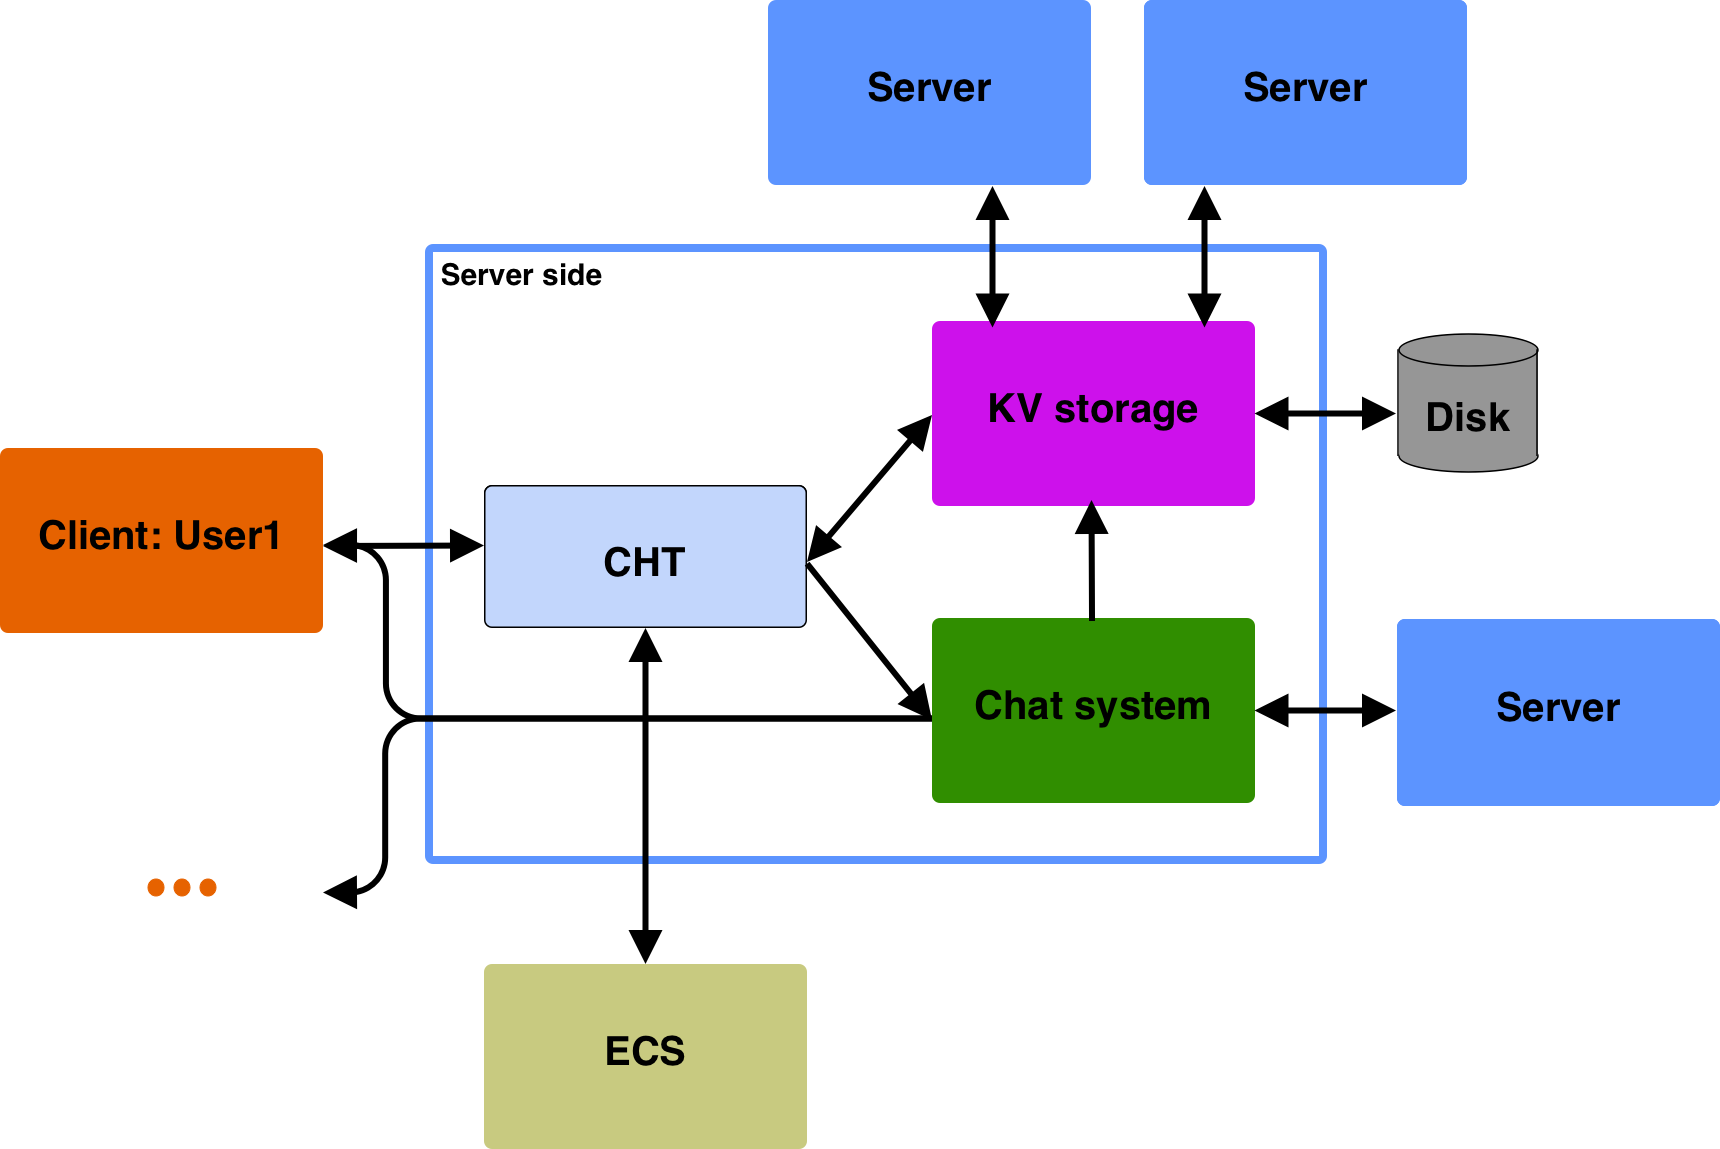
\includegraphics[width=\linewidth]{figures/chat/chat_full_arch.png}
	\caption{Server side architecture}
	\label{fig:chat_arch}
\end{figure}

In MS5, we extended our program with a group chat feature which enables clients to exchange messages with each other through chatrooms. We are able to integrate the chatting system neatly into our existing key-value server architecture, as seen in figure \ref{fig:chat_arch}. Additionally, we developed our group chat in such a way that clients can access the DB while being in a chatroom with the help of a chatbot.
 
In the following section, the basic functionalities of the group chat are described step by step, subsequently the chat system and its components are examined in depth. Lastly, we discuss how client can access the DB while chatting.

\subsection{Basic Functionalities}
\label{sec:groupchat_functionalities}
To start off, in the same sense as MS4, the External Configuration Service (ECS), where the storage servers are monitored and controlled, is started. Following that a number of servers are created. A client must connect to one of the servers.

\subsubsection{Unique Username}
\label{sec:groupchat_funtionalities_uniqueusername}
After successfully connecting to a key-value server, the client has to either enter a username or use the command \texttt{QUIT} to have a username randomly assigned to him. Usernames are implemented as globally unique identifiers for the clients, which prevents different clients from having the same username in different chatrooms. That way, users are guaranteed to know who they are communicating with, as long as their partner is connected to the system.
In order to avoid unnecessary extra connections, the ECS stores a list of users. Whenever a client connects and tries to set its username, the request gets sent through the CHT to the ECS, as depicted in \ref{fig:chat_arch}, which then checks if the username has been already taken by a client connected to any of the servers online. The end user either receives a welcome message with the username displayed if the operation was succesful, or an error message.
 
\subsubsection{Chatrooms}
\label{sec:groupchat_funtionalities_chatcommand}
In order to use to start chatting, the client has to join a chatroom. This is done by typing \texttt{chat} and providing the ID of the chatroom. In case the room does not exist, the user is allowed to create one. The next time a user executes the \texttt{chat} command with the same chatID, he is either granted access to it immediately if it is a public room, or is otherwise first required to enter the password chosen by the person who created the room. The password is hashed on the client side for safety measures and only the hash is required to validate the password attempt.
Each server owns a list containing the active chatrooms that it is responsible for depending on its position on the hash ring. In order for a client to join one of those chatrooms, is that it would first need to connect to that server, similar to the way storing key-value pair works.

\subsubsection{Saved Messages}
\label{sec:groupchat_funtionalities_savedmessages}
Messages sent in a chatroom get stored into a text file under the directory of the responsible server. We provide this feature, in case a network partition occurs in the system, so that we are able to restore messages get lost.

\subsubsection{Additional Commands}
\label{sec:groupchat_funtionalities_commands}
The \texttt{WSP} command allows a private message to be sent to multiple users.
Messages sent in the chatroom get prepended with a timestamp. Also, whenever a client joins or leaves a chatroom, all users inside get notified. This helps the user keep on track with the flow of the messages. Otherwise, users could use the \texttt{ACTIVE} command to obtain a list of all users currently in the chatroom. 

\begin{figure}[h]
	\centering
	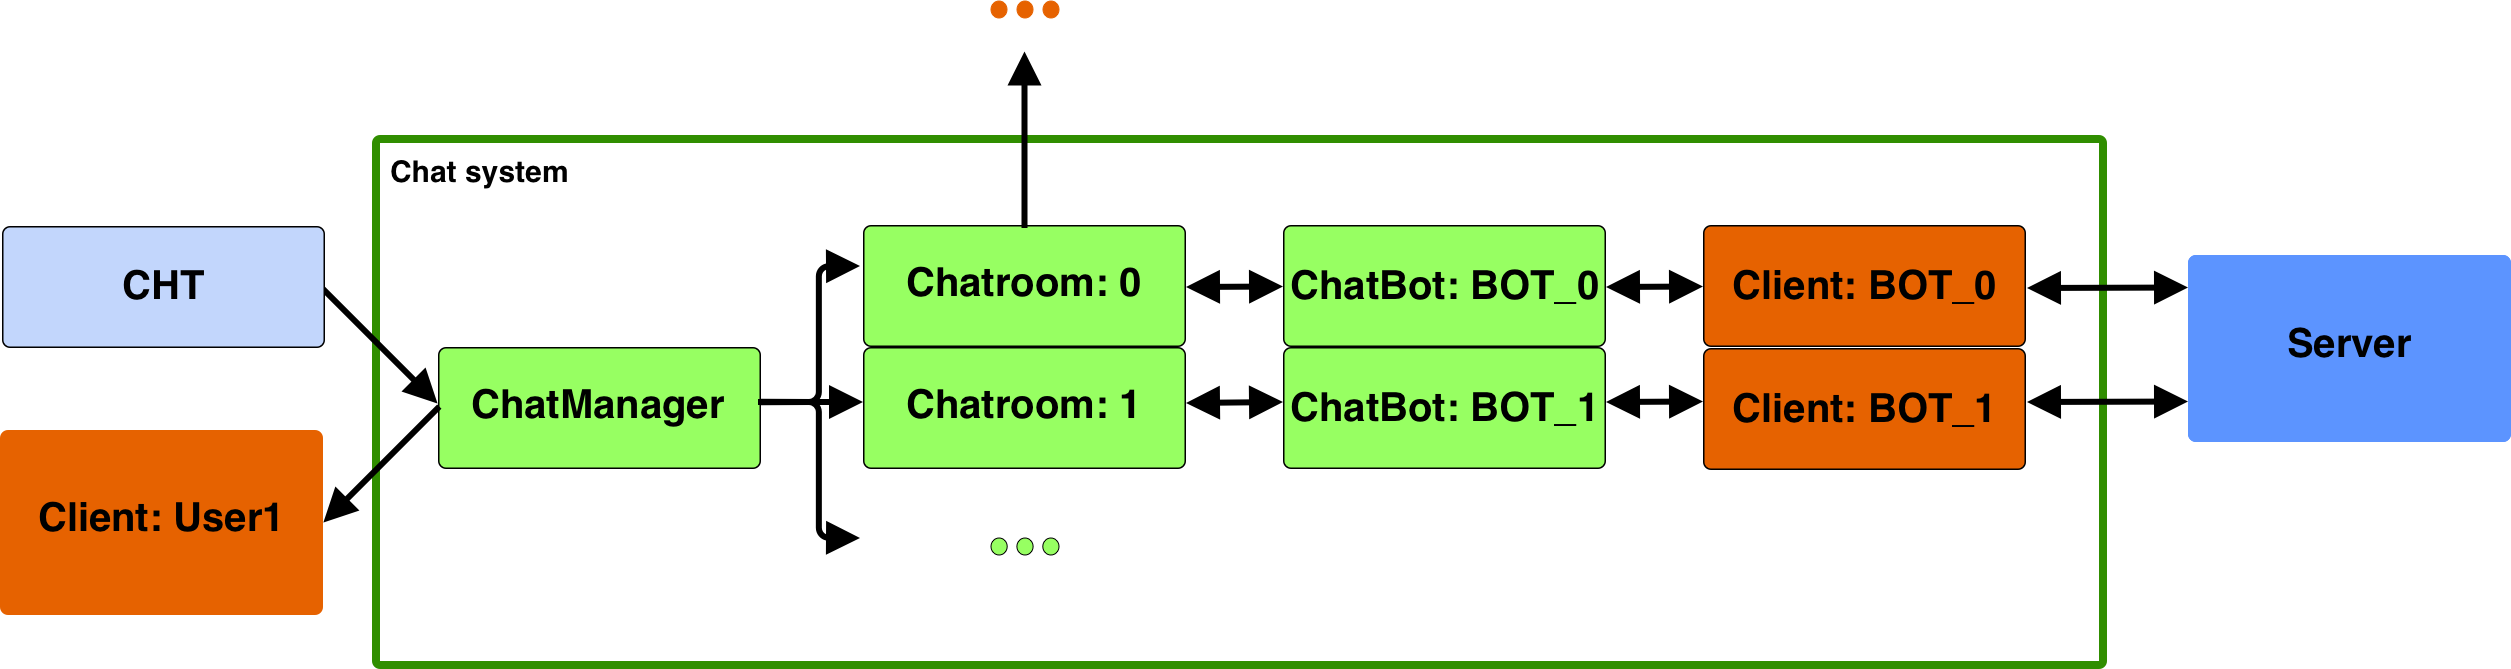
\includegraphics[width=\linewidth]{figures/chat/chat_arch.png}
	\caption{Chat system}
\end{figure}

The chat system consists of three main components as seen in the above figure\ref{fig:}:
\begin{enumerate}
	\item \textit{ChatManager}, who is in charge of providing all chat functionalities to the client, including connecting to a chatroom and sending messages.
	\item \textit{ChatRoom}, which is identified by a chatID. A Chatroom object contains a map of all connected users and their sockets, in order to be able to forward messages.
	\item \textit{ChatBot}, which is responsible to execute PUT and GET commands during a chat session. The chatbot acts exactly like a client, meaning it first has to connect to the responsible server and then send its request.

\end{enumerate}

\subsection{Database Access}
\label{sec:groupchat_chatbot}
In order to provide the chatting functionality, the server would need a socket to send to and receive messages from. However, the client also requires a socket to connect to the DB. The obvious design decision would be to add an extra socket to the client responsible for just chatting. The drawback of that idea is that the amount of TCP connections per client would get doubled, which would increase the network traffic to a large extent. In our intended use case, clients are not expected to utilize the DB heavily during chat sessions. For that reason, we could allow clients to quickly leave the chatroom to perform the DOPs and then rejoin. However, that might cause the client to miss messages while he is away, which affects the system's availability guarantee described in %TODO \ref{} server.

The approach we decided to follow in the end was creating a chatbot, whose sole purpose is executing DOPs for chat users. The chatbot acts mostly similar to a client by being able to send read and write requests to the DB. Every chatroom gets a chatbot assigned to it, which scans all incoming chat messages for DOPs, signaled by the keywords \texttt{PUT} and \texttt{GET}. Those requests are then sent to the DB and the result is returned to the chat user. In case of a read request, the \texttt{GET} operation in the message is replaced by the retrieved result. Only after this translation will the chatroom send the now modified message to every participant in the chatroom. This allows users to use stored values for communication.

delete??
%TODO delete?
chat system:
All chat related requests get transferred by the CHT to the ChatManager. This has a list of Chatroom objects. When a client tries to connect to a chatroom, the ChatManager checks the list whether a chatroom with the provided chatID already exists or not. In the former case, 
if the chatroom is public, the client is granted access or, in case of a private chatroom, requested to enter a password. In the event of no chatroom found with the given chatID, the client is allowed to create the chatroom by specifying its type and providing a password, if a private chatroom is chosen. In order to increase security, the password gets hashed on the client side and only the hash of the password is stored at the server side and used for validation.
\section{Implementation}
\label{sec:implementation}

In this section the implementation of the chatroom is examined in depth. Firstly, the extension for the client side and then for the server side are described respectively. 

\subsection{Client Side Implementation}
\label{sec:Implementation_clintside}


\subsubsection{Client Library}
\label{sec:implementation_clientside_clientlib}


 
 
\subsection{Server Side Implementation}
\label{sec:implementation_serverside}
\section{Performance Analysis}
\label{sec:perf}

After we were done with the implementation of MS5, we wanted to test our system to 1) analyze the response times of normal read and write operations, and 2) check the impact of the chatting functionality on the response times. 

320 key-value pairs are used as input for the tests, which were derived from the Enron email set. The way the test works is that clients execute \texttt{PUT}s on all keys, then they try obtaining them back with \texttt{GET}s and in the end all keys are deleted. Each of the three different operations got timed seperatly, so that their efficiency could be compared. The cache replacement strategy in place was Least Recently Used (LRU), which is the default strategy, and the cache size was set to 16, which represents 5\% of the storage size. Before a new set of commands got started, the list of keys got shuffled, which causes both the degree of cache utilization during read operations and the chance of reconnecting to the responsible server to be more or less based on luck.
In order to avoid skewed results, each test was ran five times and the average was taken.

\begin{figure}
	\begin{subfigure}[b]{\linewidth}
	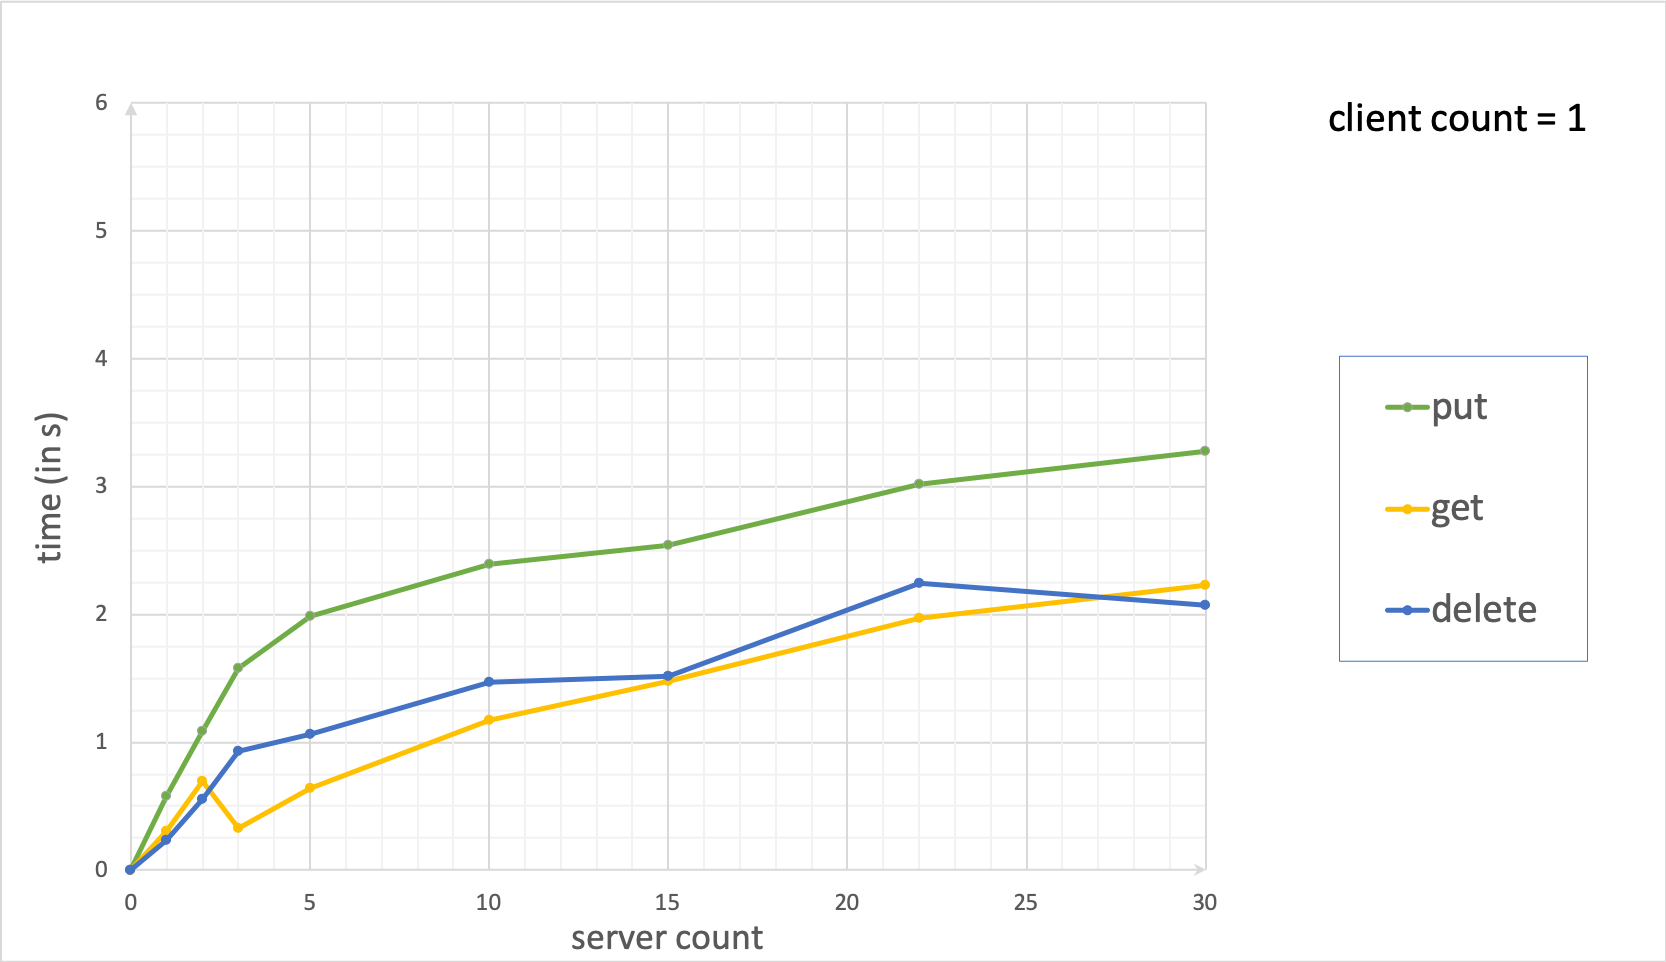
\includegraphics[width=\linewidth]{figures/cc1.png}
\caption{}
\label{fig:perf_cc1}
	\end{subfigure}
	\begin{subfigure}[b]{\linewidth}
	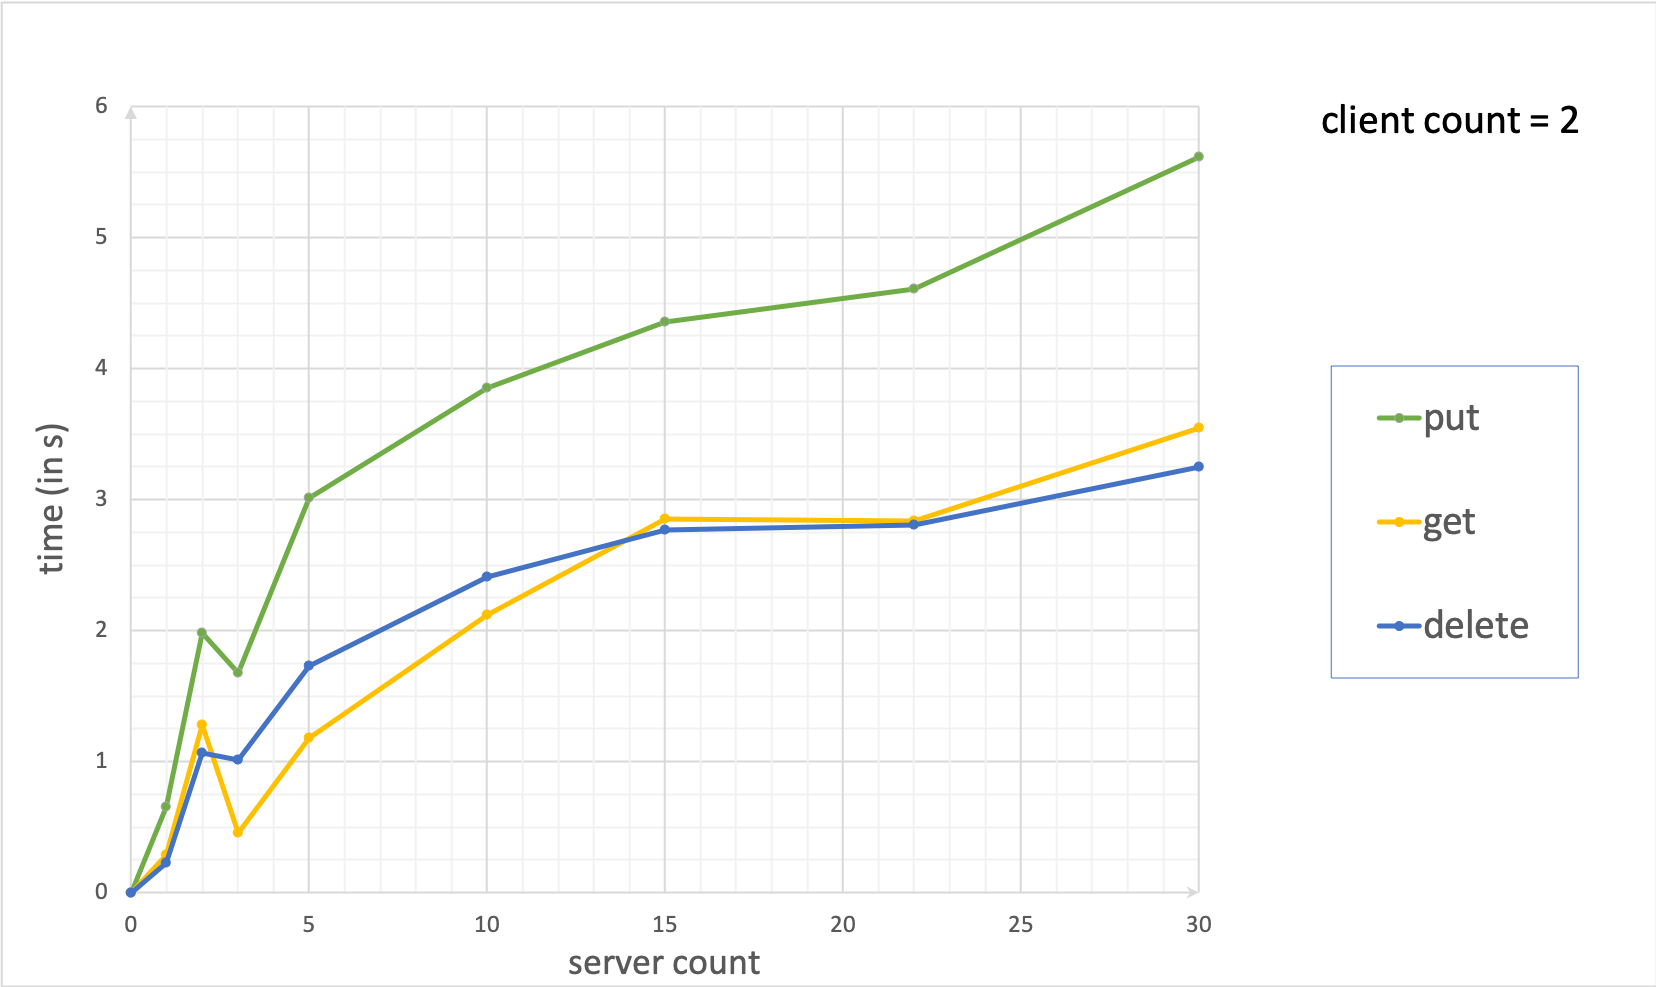
\includegraphics[width=\linewidth]{figures/cc2.png}
\caption{}
\label{fig:perf_cc2}
	\end{subfigure}
\caption{Key-value servers performance}
\label{fig:perf_cc}
\end{figure}

In figure \ref{fig:perf_cc}  we vary the amount of key-value servers and measure the time 320 operations took. At first glance, it is clear that adding an extra client in \ref{fig:perf_cc2} leads to lower response times, since double the amount of requests need to get processed by the servers. Otherwise, in both graphs \texttt{PUT} operations take the most time, because each time the disk has to be accessed and a file has to be written. Even though deletetion manipulates data on disk as well, files just have to be located and removed from the directory, with no need to open them. \texttt{GET}s usually took the least amount of time, since disk access is not always necessary. A significant drop of read response time can be noticed at the three server mark due to replication just getting started. At that point, no reconnection is required for the read commands, owing to the fact that all three servers are now responsible for read operations on all keys. The chance of a reconnection being needed is equal to \begin{math}1-\frac{3}{N}\end{math} with \begin{math}N\end{math} being the amount of key-value servers running. As apparent by the formula, the chance decreases as the server count increases, leading to the rise seen later on in the graphs. 


\begin{figure}[h]
	\centering
	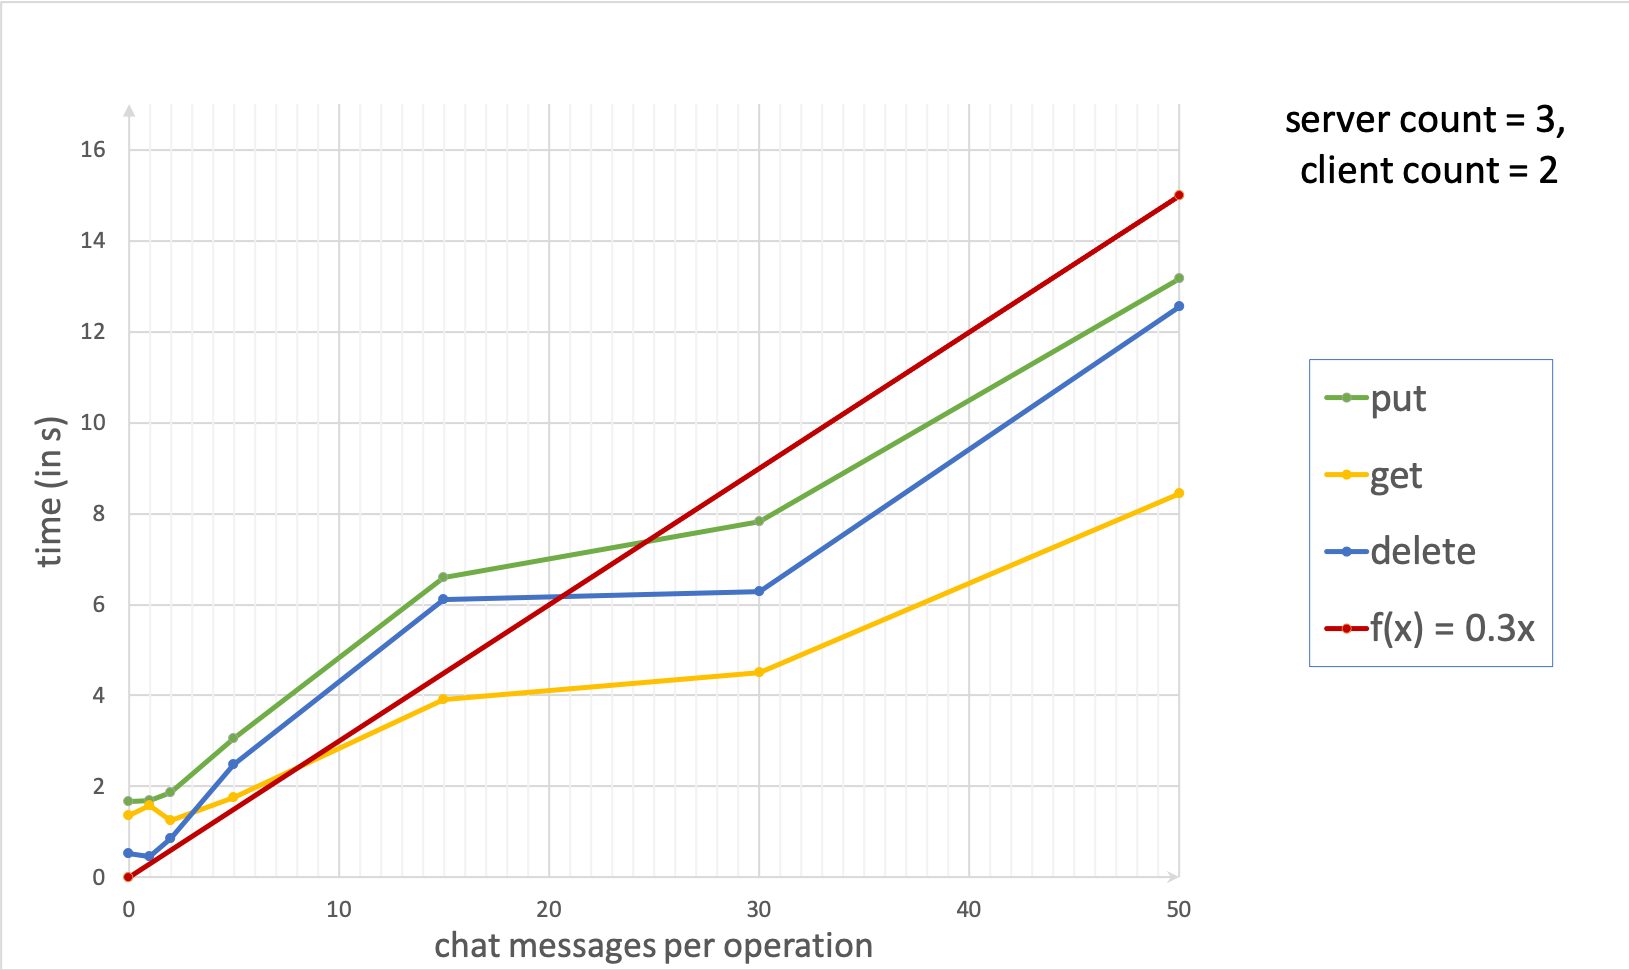
\includegraphics[width=\linewidth]{figures/chat(linear).png}
	\caption{Key-value servers performance in chat mode}
	\label{fig:perf_chat_lin}
\end{figure}

After we have evaluated the response time for the normal database operations, we try executing these same commands but inside a chatroom. For our testing purposes, we had two clients in the same chatroom perform those commands. The difference here is that, unlike in figure \ref{fig:perf_cc2}, where each client directly contacts the key-value servers, only one common bot is utilized by both users. After each command, the user would send a certain number of chat messages as depicted on the X-axis, in order to simulate a general use case scenario of our system. Graph \ref{fig:perf_chat_lin} depicts the increase in response time in relation to the chat messages sent.
When few messages are sent, the extra time required compared to the normal database operations seems unnecessary. 
However, the response times do not grow at the same ratio as the chat activity, but rather roughly follow the path of the function \begin{math}0.3x\end{math}. That means that for each additional chat message per operation per client (equal to overall \begin{math}320 * 2 = 640\end{math} extra messages), the system is slower by just about 300 milliseconds. In one extra second, more than 2100 messages can get exchanged.
\section{Summary}
\label{sec:summary}

To conclude our paper, with the group chat extension in our system we provided clients a chat system which supports low latency and high availability. We got inspired by Redis Pub/Sub strategy and adjusted it in our system by bringing the clients on the same level instead of having publishers and subscribers. As we mentioned in the motivation section \ref{sec:motivation} subscribers are waiting on an update of the subscribed key and during this process clients do not use any other functionalities in the system. To prevent the idle time which client just waits a response from the server, we enhanced the system maintaining many-to-many relationship in contrast Redis’ one-to-many relationship.

During the development process, initially we considered the demands of the client, for instance having globally unique usernames, accessing the database while chatting and having private and public chatrooms. Subsequently, with the implementation of the chat system we fulfilled the potential demands and extent it with features such as “ACTIVE” or “WSP” commands as explained in the section Newly added commands for the group chat \ref{sec:groupchat_commands}.

Consequently, after the performance tests we recommend our system for light-weighted communication. The reason for that is as explained in the Server side implementation \ref{sec:implementation_serverside} in greater detail, it might occur that the chatrooms are not equally distributed in the system and thereby just one server might have to carry the load of having all the chatrooms. And this leads us one of our so to say weaknesses in the system which is the limitations. We limited the number of chatrooms to 15 for one server and the number of users using one chatroom to 30. The numbers could be arranged depending on the use case of the system. If the user of our group chat prefers to work on a large-scaled messaging platform and can give up on having low latency, the limitations for the number of chatrooms and the clients could be increased.

One of our strengths is allowing the access to the database while clients are chatting.






\bibliographystyle{ACM-Reference-Format}
\bibliography{bibliography}

\appendix


\end{document}
\endinput


